% Options for packages loaded elsewhere
\PassOptionsToPackage{unicode}{hyperref}
\PassOptionsToPackage{hyphens}{url}
%
\documentclass[
]{article}
\usepackage{amsmath,amssymb}
\usepackage{lmodern}
\usepackage{iftex}
\ifPDFTeX
  \usepackage[T1]{fontenc}
  \usepackage[utf8]{inputenc}
  \usepackage{textcomp} % provide euro and other symbols
\else % if luatex or xetex
  \usepackage{unicode-math}
  \defaultfontfeatures{Scale=MatchLowercase}
  \defaultfontfeatures[\rmfamily]{Ligatures=TeX,Scale=1}
\fi
% Use upquote if available, for straight quotes in verbatim environments
\IfFileExists{upquote.sty}{\usepackage{upquote}}{}
\IfFileExists{microtype.sty}{% use microtype if available
  \usepackage[]{microtype}
  \UseMicrotypeSet[protrusion]{basicmath} % disable protrusion for tt fonts
}{}
\makeatletter
\@ifundefined{KOMAClassName}{% if non-KOMA class
  \IfFileExists{parskip.sty}{%
    \usepackage{parskip}
  }{% else
    \setlength{\parindent}{0pt}
    \setlength{\parskip}{6pt plus 2pt minus 1pt}}
}{% if KOMA class
  \KOMAoptions{parskip=half}}
\makeatother
\usepackage{xcolor}
\usepackage[margin=1in]{geometry}
\usepackage{color}
\usepackage{fancyvrb}
\newcommand{\VerbBar}{|}
\newcommand{\VERB}{\Verb[commandchars=\\\{\}]}
\DefineVerbatimEnvironment{Highlighting}{Verbatim}{commandchars=\\\{\}}
% Add ',fontsize=\small' for more characters per line
\usepackage{framed}
\definecolor{shadecolor}{RGB}{248,248,248}
\newenvironment{Shaded}{\begin{snugshade}}{\end{snugshade}}
\newcommand{\AlertTok}[1]{\textcolor[rgb]{0.94,0.16,0.16}{#1}}
\newcommand{\AnnotationTok}[1]{\textcolor[rgb]{0.56,0.35,0.01}{\textbf{\textit{#1}}}}
\newcommand{\AttributeTok}[1]{\textcolor[rgb]{0.77,0.63,0.00}{#1}}
\newcommand{\BaseNTok}[1]{\textcolor[rgb]{0.00,0.00,0.81}{#1}}
\newcommand{\BuiltInTok}[1]{#1}
\newcommand{\CharTok}[1]{\textcolor[rgb]{0.31,0.60,0.02}{#1}}
\newcommand{\CommentTok}[1]{\textcolor[rgb]{0.56,0.35,0.01}{\textit{#1}}}
\newcommand{\CommentVarTok}[1]{\textcolor[rgb]{0.56,0.35,0.01}{\textbf{\textit{#1}}}}
\newcommand{\ConstantTok}[1]{\textcolor[rgb]{0.00,0.00,0.00}{#1}}
\newcommand{\ControlFlowTok}[1]{\textcolor[rgb]{0.13,0.29,0.53}{\textbf{#1}}}
\newcommand{\DataTypeTok}[1]{\textcolor[rgb]{0.13,0.29,0.53}{#1}}
\newcommand{\DecValTok}[1]{\textcolor[rgb]{0.00,0.00,0.81}{#1}}
\newcommand{\DocumentationTok}[1]{\textcolor[rgb]{0.56,0.35,0.01}{\textbf{\textit{#1}}}}
\newcommand{\ErrorTok}[1]{\textcolor[rgb]{0.64,0.00,0.00}{\textbf{#1}}}
\newcommand{\ExtensionTok}[1]{#1}
\newcommand{\FloatTok}[1]{\textcolor[rgb]{0.00,0.00,0.81}{#1}}
\newcommand{\FunctionTok}[1]{\textcolor[rgb]{0.00,0.00,0.00}{#1}}
\newcommand{\ImportTok}[1]{#1}
\newcommand{\InformationTok}[1]{\textcolor[rgb]{0.56,0.35,0.01}{\textbf{\textit{#1}}}}
\newcommand{\KeywordTok}[1]{\textcolor[rgb]{0.13,0.29,0.53}{\textbf{#1}}}
\newcommand{\NormalTok}[1]{#1}
\newcommand{\OperatorTok}[1]{\textcolor[rgb]{0.81,0.36,0.00}{\textbf{#1}}}
\newcommand{\OtherTok}[1]{\textcolor[rgb]{0.56,0.35,0.01}{#1}}
\newcommand{\PreprocessorTok}[1]{\textcolor[rgb]{0.56,0.35,0.01}{\textit{#1}}}
\newcommand{\RegionMarkerTok}[1]{#1}
\newcommand{\SpecialCharTok}[1]{\textcolor[rgb]{0.00,0.00,0.00}{#1}}
\newcommand{\SpecialStringTok}[1]{\textcolor[rgb]{0.31,0.60,0.02}{#1}}
\newcommand{\StringTok}[1]{\textcolor[rgb]{0.31,0.60,0.02}{#1}}
\newcommand{\VariableTok}[1]{\textcolor[rgb]{0.00,0.00,0.00}{#1}}
\newcommand{\VerbatimStringTok}[1]{\textcolor[rgb]{0.31,0.60,0.02}{#1}}
\newcommand{\WarningTok}[1]{\textcolor[rgb]{0.56,0.35,0.01}{\textbf{\textit{#1}}}}
\usepackage{longtable,booktabs,array}
\usepackage{calc} % for calculating minipage widths
% Correct order of tables after \paragraph or \subparagraph
\usepackage{etoolbox}
\makeatletter
\patchcmd\longtable{\par}{\if@noskipsec\mbox{}\fi\par}{}{}
\makeatother
% Allow footnotes in longtable head/foot
\IfFileExists{footnotehyper.sty}{\usepackage{footnotehyper}}{\usepackage{footnote}}
\makesavenoteenv{longtable}
\usepackage{graphicx}
\makeatletter
\def\maxwidth{\ifdim\Gin@nat@width>\linewidth\linewidth\else\Gin@nat@width\fi}
\def\maxheight{\ifdim\Gin@nat@height>\textheight\textheight\else\Gin@nat@height\fi}
\makeatother
% Scale images if necessary, so that they will not overflow the page
% margins by default, and it is still possible to overwrite the defaults
% using explicit options in \includegraphics[width, height, ...]{}
\setkeys{Gin}{width=\maxwidth,height=\maxheight,keepaspectratio}
% Set default figure placement to htbp
\makeatletter
\def\fps@figure{htbp}
\makeatother
\setlength{\emergencystretch}{3em} % prevent overfull lines
\providecommand{\tightlist}{%
  \setlength{\itemsep}{0pt}\setlength{\parskip}{0pt}}
\setcounter{secnumdepth}{-\maxdimen} % remove section numbering
\ifLuaTeX
  \usepackage{selnolig}  % disable illegal ligatures
\fi
\IfFileExists{bookmark.sty}{\usepackage{bookmark}}{\usepackage{hyperref}}
\IfFileExists{xurl.sty}{\usepackage{xurl}}{} % add URL line breaks if available
\urlstyle{same} % disable monospaced font for URLs
\hypersetup{
  pdftitle={project 1 markdown},
  pdfauthor={Joey Hernandez and Robert Blue},
  hidelinks,
  pdfcreator={LaTeX via pandoc}}

\title{project 1 markdown}
\author{Joey Hernandez and Robert Blue}
\date{2022-10-18}

\begin{document}
\maketitle

\hypertarget{introduction}{%
\subsection{Introduction:}\label{introduction}}

\hypertarget{thank-you-mr.smith-and-mr.-jones-for-the-opportunity-for-us-to-deliver-beer-and-brewery-insights-so-that-your-company-booze-and-brews-can-align-its-strategic-plan-for-growth-and-future-offerings-so-that-you-can-maximize-revenues-and-grow-your-presence.}{%
\paragraph{Thank you Mr.Smith, and Mr.~Jones for the opportunity for us
to deliver Beer and Brewery insights so that your company Booze and
Brews can align it's strategic plan for growth, and future offerings so
that you can maximize revenues and grow your
presence.}\label{thank-you-mr.smith-and-mr.-jones-for-the-opportunity-for-us-to-deliver-beer-and-brewery-insights-so-that-your-company-booze-and-brews-can-align-its-strategic-plan-for-growth-and-future-offerings-so-that-you-can-maximize-revenues-and-grow-your-presence.}}

\hypertarget{it-was-a-pleasure-working-with-you-and-your-team-and-we-hope-you-are-able-to-gain-strong-insights-from-our-analysis-of-the-data-you-provided-us.}{%
\paragraph{It was a pleasure working with you and your team, and we hope
you are able to gain strong insights from our analysis of the data you
provided
us.}\label{it-was-a-pleasure-working-with-you-and-your-team-and-we-hope-you-are-able-to-gain-strong-insights-from-our-analysis-of-the-data-you-provided-us.}}

The first step in our process is to load the data and necessary
libraries so that we can investigate the data with a full assortment of
tools needed to present our findings base on the beer and breweries
data.

\begin{Shaded}
\begin{Highlighting}[]
\FunctionTok{library}\NormalTok{(tidyverse)}
\end{Highlighting}
\end{Shaded}

\begin{verbatim}
## -- Attaching packages --------------------------------------- tidyverse 1.3.2 --
## v ggplot2 3.3.6     v purrr   0.3.4
## v tibble  3.1.8     v dplyr   1.0.9
## v tidyr   1.2.0     v stringr 1.4.1
## v readr   2.1.2     v forcats 0.5.1
## -- Conflicts ------------------------------------------ tidyverse_conflicts() --
## x dplyr::filter() masks stats::filter()
## x dplyr::lag()    masks stats::lag()
\end{verbatim}

\begin{Shaded}
\begin{Highlighting}[]
\FunctionTok{library}\NormalTok{(ggplot2)}
\FunctionTok{library}\NormalTok{(janitor)}
\end{Highlighting}
\end{Shaded}

\begin{verbatim}
## 
## Attaching package: 'janitor'
## 
## The following objects are masked from 'package:stats':
## 
##     chisq.test, fisher.test
\end{verbatim}

\begin{Shaded}
\begin{Highlighting}[]
\FunctionTok{library}\NormalTok{(usmap)}
\FunctionTok{library}\NormalTok{(caret)}
\end{Highlighting}
\end{Shaded}

\begin{verbatim}
## Loading required package: lattice
## 
## Attaching package: 'caret'
## 
## The following object is masked from 'package:purrr':
## 
##     lift
\end{verbatim}

\begin{Shaded}
\begin{Highlighting}[]
\FunctionTok{library}\NormalTok{(e1071)}
\FunctionTok{library}\NormalTok{(class)}
\FunctionTok{library}\NormalTok{(knitr)}
\FunctionTok{library}\NormalTok{(ggthemes)}
\NormalTok{beer\_data }\OtherTok{\textless{}{-}}\FunctionTok{read.csv}\NormalTok{(}\StringTok{"C:/Users/Joey/Desktop/DDS\_Work/Unit {-} 8/Beers.csv"}\NormalTok{)}
\NormalTok{brew\_data }\OtherTok{\textless{}{-}} \FunctionTok{read.csv}\NormalTok{(}\StringTok{"C:/Users/Joey/Desktop/DDS\_Work/Unit {-} 8/Breweries.csv"}\NormalTok{)}
\end{Highlighting}
\end{Shaded}

\hypertarget{question-of-interest-1---data-at-a-glance-missing-vaules}{%
\subsection{Question of Interest 1 - Data at a glance \& Missing
Vaules}\label{question-of-interest-1---data-at-a-glance-missing-vaules}}

\hypertarget{during-our-initial-consultation-you-mentioned-the-data-could-contain-some-missing-values-as-well-as-some-potential-errors.-in-order-for-us-to-present-the-most-accurate-findings-we-took-a-series-of-steps-to-ensure-that-any-errors-or-missing-values-were-either-addressed-or-corrected.}{%
\paragraph{During our initial consultation, you mentioned the data could
contain some missing values as well as some potential errors. In order
for us to present the most accurate findings, we took a series of steps
to ensure that any errors or missing values were either addressed or
corrected.}\label{during-our-initial-consultation-you-mentioned-the-data-could-contain-some-missing-values-as-well-as-some-potential-errors.-in-order-for-us-to-present-the-most-accurate-findings-we-took-a-series-of-steps-to-ensure-that-any-errors-or-missing-values-were-either-addressed-or-corrected.}}

\hypertarget{identify-the-rows-and-columns-of-the-data-sets.-this-first-glance-allows-us-to-understand-what-type-of-variables-and-variable-types-we-are-working-with-additionally-we-are-able-to-understand-the-size-of-data-that-we-have.}{%
\subparagraph{1. Identify the rows and columns of the data sets. This
first glance allows us to understand what type of variables and variable
types we are working with, additionally, we are able to understand the
size of data that we
have.}\label{identify-the-rows-and-columns-of-the-data-sets.-this-first-glance-allows-us-to-understand-what-type-of-variables-and-variable-types-we-are-working-with-additionally-we-are-able-to-understand-the-size-of-data-that-we-have.}}

\hypertarget{viewing-the-datasets-allowed-us-to-identify-similar-columns-within-the-2-groups-that-we-could-use-to-merge-the-data.-merging-the-data-together-allows-us-to-create-a-dataframe-that-contains-all-we-need-in-one-location.-we-will-not-yet-merge-the-data-within-this-step-but-we-do-take-action-and-rename-any-columns-that-may-be-of-intrest.-what-you-will-find-if-you-look-at-the-data-is-that-we-changed-both-data-brewery-identification-columns-to-the-title-brewery_id-so-that-we-could-merge-the-data-with-this-as-our-bridge-variable.}{%
\subparagraph{2. Viewing the datasets allowed us to identify similar
columns within the 2 groups that we could use to merge the data. Merging
the data together allows us to create a dataframe that contains all we
need in one location. We will not yet merge the data within this step
but we do take action and rename any columns that may be of intrest.
What you will find if you look at the data is that we changed both data
brewery identification columns to the title `Brewery\_id' so that we
could merge the data with this as our bridge
variable.}\label{viewing-the-datasets-allowed-us-to-identify-similar-columns-within-the-2-groups-that-we-could-use-to-merge-the-data.-merging-the-data-together-allows-us-to-create-a-dataframe-that-contains-all-we-need-in-one-location.-we-will-not-yet-merge-the-data-within-this-step-but-we-do-take-action-and-rename-any-columns-that-may-be-of-intrest.-what-you-will-find-if-you-look-at-the-data-is-that-we-changed-both-data-brewery-identification-columns-to-the-title-brewery_id-so-that-we-could-merge-the-data-with-this-as-our-bridge-variable.}}

\hypertarget{before-merging-the-data-together-we-checked-each-dataset-individually-for-missing-values-and-broke-them-into-explicit-and-implicit-missing-values.}{%
\subparagraph{3. Before merging the data together we checked each
dataset individually for missing values and broke them into explicit and
implicit missing
values.}\label{before-merging-the-data-together-we-checked-each-dataset-individually-for-missing-values-and-broke-them-into-explicit-and-implicit-missing-values.}}

\hypertarget{we-addressed-explicit-values-nas-by-investigating-why-there-may-have-been-expliciltly-missing-values-in-the-data.-upon-further-investigation-we-discovered-that-certain-values-are-not-always-reported-or-are-required-to-be-reported-by-breweries.-this-varies-from-brewery-to-brewery-but-most-often-has-to-do-with-state-and-other-governing-matters.-in-the-case-of-missing-ibu-values-this-also-varies-from-location-to-location-and-can-be-attributed-to-differnent-crafting-methods-in-addition-to-simply-not-being-required-to-report.-we-did-not-completely-leave-out-this-data-but-instead-left-it-as-na-when-applicaple-since-it-represented-such-a-high-amount-of-data.}{%
\subparagraph{4. We addressed Explicit Values (NAs) by investigating why
there may have been expliciltly missing values in the data. Upon further
investigation we discovered that certain values are not always reported
(or are required to be reported) by breweries. This varies from brewery
to brewery but most often has to do with state and other governing
matters. In the case of missing IBU values this also varies from
location to location and can be attributed to differnent crafting
methods in addition to simply not being required to report. We did not
completely leave out this data, but instead left it as NA when
applicaple since it represented such a high amount of
data.}\label{we-addressed-explicit-values-nas-by-investigating-why-there-may-have-been-expliciltly-missing-values-in-the-data.-upon-further-investigation-we-discovered-that-certain-values-are-not-always-reported-or-are-required-to-be-reported-by-breweries.-this-varies-from-brewery-to-brewery-but-most-often-has-to-do-with-state-and-other-governing-matters.-in-the-case-of-missing-ibu-values-this-also-varies-from-location-to-location-and-can-be-attributed-to-differnent-crafting-methods-in-addition-to-simply-not-being-required-to-report.-we-did-not-completely-leave-out-this-data-but-instead-left-it-as-na-when-applicaple-since-it-represented-such-a-high-amount-of-data.}}

\hypertarget{the-data-did-contain-some-implicit-values-in-the-form-of-missing-data.-upon-futher-investigation-we-were-able-to-either-remedy-the-missing-values-by-researching-the-product-in-question-or-gain-an-understanding-of-why-a-value-may-not-have-been-present-so-that-we-could-understand-how-it-would-impact-the-remaning-data-or-if-it-impacted-the-remaining-data.}{%
\subparagraph{5. The data did contain some Implicit values in the form
of missing data. Upon futher investigation we were able to either remedy
the missing values by researching the product in question, or gain an
understanding of why a value may not have been present so that we could
understand how it would impact the remaning data (or if it impacted the
remaining
data).}\label{the-data-did-contain-some-implicit-values-in-the-form-of-missing-data.-upon-futher-investigation-we-were-able-to-either-remedy-the-missing-values-by-researching-the-product-in-question-or-gain-an-understanding-of-why-a-value-may-not-have-been-present-so-that-we-could-understand-how-it-would-impact-the-remaning-data-or-if-it-impacted-the-remaining-data.}}

\hypertarget{there-was-instances-of-duplicate-data-which-were-attributed-to-incorrect-brewery-locations-or-were-attributed-to-repeated-batches-of-an-offering-as-well-as-different-sizes-of-certain-drinks.-the-remedy-was-addressed-on-a-case-by-case-basis-but-in-short-the-only-data-removed-was-data-that-was-incorrect-such-as-the-duplicate-locations-entered-by-spelling-or-typo-errors.}{%
\subparagraph{6. There was instances of duplicate data which were
attributed to incorrect brewery locations, or were attributed to
repeated batches of an offering as well as different sizes of certain
drinks. The remedy was addressed on a case by case basis, but in short
the only data removed was data that was incorrect, such as the duplicate
locations entered by spelling, or typo
errors.}\label{there-was-instances-of-duplicate-data-which-were-attributed-to-incorrect-brewery-locations-or-were-attributed-to-repeated-batches-of-an-offering-as-well-as-different-sizes-of-certain-drinks.-the-remedy-was-addressed-on-a-case-by-case-basis-but-in-short-the-only-data-removed-was-data-that-was-incorrect-such-as-the-duplicate-locations-entered-by-spelling-or-typo-errors.}}

\hypertarget{while-not-a-big-issue-the-state-abbreviations-all-contained-some-white-space-before-the-actual-charater-of-the-string.-this-white-space-was-removed-to-better-utilize-the-variable.}{%
\subparagraph{7. While not a big issue, the state abbreviations all
contained some white space before the actual charater of the string.
This white space was removed to better utilize the
variable.}\label{while-not-a-big-issue-the-state-abbreviations-all-contained-some-white-space-before-the-actual-charater-of-the-string.-this-white-space-was-removed-to-better-utilize-the-variable.}}

\hypertarget{finally-after-all-found-errors-were-addressed-we-merged-the-data-into-one-piece.}{%
\subparagraph{8. Finally after all found errors were addressed, we
merged the data into one
piece.}\label{finally-after-all-found-errors-were-addressed-we-merged-the-data-into-one-piece.}}

\begin{Shaded}
\begin{Highlighting}[]
\DocumentationTok{\#\#\#\#\#\#\#\#\#\#\#\#\#\#\#\#\#\#\#\# Exploring Raw Data \#\#\#\#\#\#\#\#\#\#\#\#\#\#\#\#\#\#\#\#\#\#\#\#\#\#\#}
\CommentTok{\# check rows and columns}
\CommentTok{\# head(beer\_data)}
\CommentTok{\# head(brew\_data)}

\CommentTok{\# rename columns for merging }
\FunctionTok{names}\NormalTok{(beer\_data)[}\DecValTok{1}\NormalTok{] }\OtherTok{\textless{}{-}} \StringTok{\textquotesingle{}beer\_name\textquotesingle{}}
\FunctionTok{names}\NormalTok{(brew\_data)[}\DecValTok{2}\NormalTok{] }\OtherTok{\textless{}{-}} \StringTok{\textquotesingle{}Brew\_name\textquotesingle{}}
\FunctionTok{names}\NormalTok{(brew\_data)[}\DecValTok{1}\NormalTok{]}\OtherTok{\textless{}{-}} \StringTok{\textquotesingle{}Brewery\_id\textquotesingle{}}


\CommentTok{\# checking for missing values beer }
\CommentTok{\# sapply(beer\_data,function(x) sum(is.na(x))/nrow(beer\_data))}
\CommentTok{\# sapply(beer\_data,function(x) sum(x== ""))}

\CommentTok{\# checking for missing values brew}
\CommentTok{\# sapply(brew\_data,function(x) sum(is.na(x))/nrow(brew\_data))}
\CommentTok{\# sapply(brew\_data,function(x) sum(x== ""))}

\CommentTok{\# addressing the missing values from beer}
\NormalTok{beer\_data[}\DecValTok{854}\NormalTok{,}\StringTok{\textquotesingle{}Style\textquotesingle{}}\NormalTok{] }\OtherTok{=} \StringTok{"Scottish Ale"}
\NormalTok{beer\_data[}\DecValTok{867}\NormalTok{, }\StringTok{\textquotesingle{}Style\textquotesingle{}}\NormalTok{] }\OtherTok{=} \StringTok{\textquotesingle{}Marzen\textquotesingle{}}



\CommentTok{\# looking for duplicates in data }
\CommentTok{\# brew\_data \%\textgreater{}\% get\_dupes(Brewery\_id)}
\CommentTok{\# brew\_data \%\textgreater{}\% get\_dupes(Brew\_name)}
\CommentTok{\# beer\_data \%\textgreater{}\% get\_dupes(beer\_name)}
\CommentTok{\# beer\_data \%\textgreater{}\% get\_dupes(Brewery\_id)}
\CommentTok{\# beer\_data \%\textgreater{}\% get\_dupes(Beer\_ID)}

\CommentTok{\# addresses the duplicates in brew\_data }
\NormalTok{brew\_data}\OtherTok{\textless{}{-}}\NormalTok{ brew\_data[}\SpecialCharTok{{-}}\FunctionTok{c}\NormalTok{(}\DecValTok{96}\NormalTok{,}\DecValTok{378}\NormalTok{,}\DecValTok{262}\NormalTok{,}\DecValTok{139}\NormalTok{),] }

\CommentTok{\# addresses the duplicates in beer\_data}
\NormalTok{beer }\OtherTok{\textless{}{-}}\NormalTok{ beer\_data[}\SpecialCharTok{!}\FunctionTok{duplicated}\NormalTok{(beer\_data}\SpecialCharTok{$}\NormalTok{beer\_name),]}
\CommentTok{\# beer \%\textgreater{}\% get\_dupes(Brewery\_id) \# these duplicates are for various drinks from the same brew id}
\CommentTok{\# beer \%\textgreater{}\% get\_dupes(Beer\_ID) \# fixed}
\CommentTok{\# beer \%\textgreater{}\% get\_dupes(beer\_name)}

\CommentTok{\# gets rid of the white space before the State abb. }
\NormalTok{brew\_data}\SpecialCharTok{$}\NormalTok{State}\OtherTok{\textless{}{-}}\FunctionTok{trimws}\NormalTok{(brew\_data}\SpecialCharTok{$}\NormalTok{State, }\StringTok{"left"}\NormalTok{)}


\CommentTok{\# merging beer and brew\_data {-} with an inner join}
\NormalTok{beer\_brew }\OtherTok{\textless{}{-}} \FunctionTok{merge}\NormalTok{(brew\_data, beer, }\AttributeTok{by =}\StringTok{\textquotesingle{}Brewery\_id\textquotesingle{}}\NormalTok{)}
\end{Highlighting}
\end{Shaded}

\hypertarget{question-of-interest}{%
\subsection{Question of Interest:}\label{question-of-interest}}

\hypertarget{how-many-breweries-are-in-each-state}{%
\paragraph{How many breweries are in each
state?}\label{how-many-breweries-are-in-each-state}}

In order to represent and visually display this data, we first had to
ensure that any duplicated values that would throw off the count for
each state were handled. Next we grouped the variables of the data into
a filtered set that we could call on to create our plot, and finally we
plotted a map of the United States the Numerical brewery representation
over each state. This type of plot intuitively shows where and how the
brewery locations are distributed across the United States. Below you
will find this breakdown visual as well as a table of the result for a
list of comparisons.

\begin{Shaded}
\begin{Highlighting}[]
\DocumentationTok{\#\#\#\#\#\#\#\#\#\#\#\#\#\#\#\#\#\#\#\#\#\#\#\#\#\#\#\#\#\#\#\#\#\#\# Question 1 \#\#\#\#\#\#\#\#\#\#\#\#\#\#\#\#\#\#\#\#\#\#\#\#\#\#\#\#\#\#\#\#\#\#}

\CommentTok{\# this gets only one brewery name so that we don\textquotesingle{}t have multiple brew representation because }
\CommentTok{\# of the multiple drinks served by that one location. }
\NormalTok{state\_num\_data }\OtherTok{\textless{}{-}}\NormalTok{ beer\_brew[}\SpecialCharTok{!}\FunctionTok{duplicated}\NormalTok{(beer\_brew}\SpecialCharTok{$}\NormalTok{Brew\_name),]}

\CommentTok{\# the n\_distinct takes care of the potential repeat brew representation making last line redundant}
\CommentTok{\# but kept in as precautionary measure.}
\NormalTok{state\_brew\_plot }\OtherTok{\textless{}{-}}\NormalTok{ state\_num\_data }\SpecialCharTok{\%\textgreater{}\%} \FunctionTok{group\_by}\NormalTok{(State) }\SpecialCharTok{\%\textgreater{}\%}
  \FunctionTok{summarise}\NormalTok{(}\AttributeTok{num\_brew =} \FunctionTok{n\_distinct}\NormalTok{(Brew\_name),}
  \AttributeTok{mean\_abv =} \FunctionTok{mean}\NormalTok{(ABV), }\AttributeTok{mean\_ibu =} \FunctionTok{mean}\NormalTok{(IBU)) }\SpecialCharTok{\%\textgreater{}\%}
  \FunctionTok{arrange}\NormalTok{(}\FunctionTok{desc}\NormalTok{(num\_brew))}

\CommentTok{\# changes column State to state to satisfy the usmap argument}
\FunctionTok{names}\NormalTok{(state\_brew\_plot)[}\DecValTok{1}\NormalTok{] }\OtherTok{\textless{}{-}} \StringTok{\textquotesingle{}state\textquotesingle{}}

\CommentTok{\# makes into dataframe}
\NormalTok{state\_brew\_plot }\OtherTok{\textless{}{-}} \FunctionTok{as.data.frame}\NormalTok{(state\_brew\_plot)}

\CommentTok{\# plot of the Concentration of Breweries in the US}
\FunctionTok{plot\_usmap}\NormalTok{(}\AttributeTok{data=}\NormalTok{state\_brew\_plot[,}\DecValTok{1}\SpecialCharTok{:}\DecValTok{2}\NormalTok{],}
           \AttributeTok{regions =} \StringTok{"states"}\NormalTok{,}
           \AttributeTok{labels =} \ConstantTok{TRUE}\NormalTok{,}\AttributeTok{label\_color =} \StringTok{"black"}\NormalTok{,}
           \AttributeTok{values =} \StringTok{"num\_brew"}\NormalTok{) }\SpecialCharTok{+}
          \FunctionTok{scale\_fill\_gradient}\NormalTok{(}\AttributeTok{low =} \StringTok{\textquotesingle{}white\textquotesingle{}}\NormalTok{, }\AttributeTok{high =} \StringTok{\textquotesingle{}red\textquotesingle{}}\NormalTok{)}\SpecialCharTok{+}
          \FunctionTok{labs}\NormalTok{(}\AttributeTok{title =} \StringTok{\textquotesingle{}Distribution of Breweries across the United States\textquotesingle{}}\NormalTok{,}
               \AttributeTok{fill =} \StringTok{"Brewery }\SpecialCharTok{\textbackslash{}n}\StringTok{Amount"}\NormalTok{) }\SpecialCharTok{+}
          \FunctionTok{theme}\NormalTok{(}\AttributeTok{legend.position =} \StringTok{"right"}\NormalTok{) }
\end{Highlighting}
\end{Shaded}

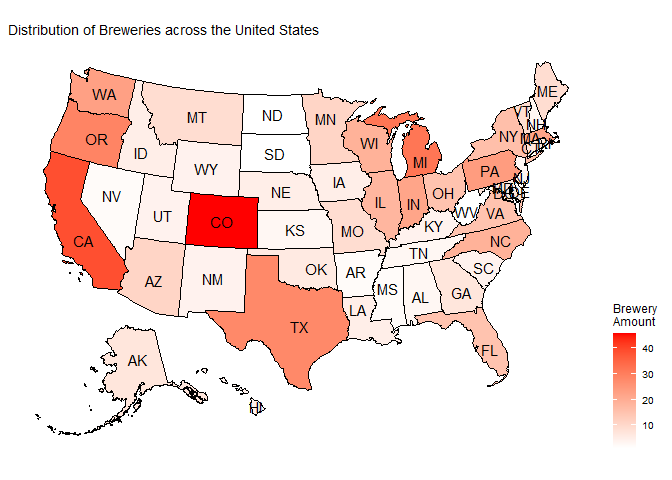
\includegraphics{ProjectMarkdown_files/figure-latex/unnamed-chunk-3-1.pdf}

\begin{Shaded}
\begin{Highlighting}[]
\CommentTok{\# SECONDARY MAP TO DISPLAY ACTUAL REPRESENTAION OF NUMERICAL VALUE PER EACH STATE }
\CommentTok{\# get centroids }
\NormalTok{centroid\_labels }\OtherTok{\textless{}{-}}\NormalTok{ usmapdata}\SpecialCharTok{::}\FunctionTok{centroid\_labels}\NormalTok{(}\StringTok{"states"}\NormalTok{)}

\FunctionTok{names}\NormalTok{(centroid\_labels)[}\DecValTok{4}\NormalTok{] }\OtherTok{\textless{}{-}} \StringTok{\textquotesingle{}state\textquotesingle{}}

\CommentTok{\# join data to centroids (using lat/long as coord. for state centers on map plot)}
\NormalTok{data\_labels }\OtherTok{\textless{}{-}} \FunctionTok{merge}\NormalTok{(centroid\_labels, state\_brew\_plot, }\AttributeTok{by =} \StringTok{"state"}\NormalTok{)}

\CommentTok{\# create US map with centroids and lat/long as the label}
\NormalTok{brews\_per\_state }\OtherTok{\textless{}{-}} \FunctionTok{plot\_usmap}\NormalTok{(}\AttributeTok{data =}\NormalTok{ state\_brew\_plot[,}\DecValTok{1}\SpecialCharTok{:}\DecValTok{2}\NormalTok{],}
                              \AttributeTok{values =} \StringTok{"num\_brew"}\NormalTok{,}
                              \AttributeTok{color =} \StringTok{"black"}\NormalTok{,}
                              \AttributeTok{labels =}\NormalTok{ F) }\SpecialCharTok{+}
  \FunctionTok{guides}\NormalTok{(}\AttributeTok{fill =} \StringTok{"none"}\NormalTok{) }\SpecialCharTok{+}
  \FunctionTok{geom\_text}\NormalTok{(}\AttributeTok{data =}\NormalTok{ data\_labels,}\FunctionTok{aes}\NormalTok{(}\AttributeTok{x =}\NormalTok{ x, }\AttributeTok{y =}\NormalTok{ y,}
                                   \AttributeTok{label =}\NormalTok{ scales}\SpecialCharTok{::}\FunctionTok{number}\NormalTok{(num\_brew, }\AttributeTok{accuracy =} \DecValTok{1}\NormalTok{)),}\AttributeTok{color =} \StringTok{"black"}\NormalTok{)}\SpecialCharTok{+} 
  \FunctionTok{scale\_fill\_gradient}\NormalTok{(}\AttributeTok{low =} \StringTok{"white"}\NormalTok{, }\AttributeTok{high =} \StringTok{"red"}\NormalTok{) }\SpecialCharTok{+}
  \FunctionTok{labs}\NormalTok{(}\AttributeTok{title =} \StringTok{"Distribution of Breweries Across The United States"}\NormalTok{,}
       \AttributeTok{fill =} \StringTok{"Brewery }\SpecialCharTok{\textbackslash{}n}\StringTok{Amount"}\NormalTok{) }\SpecialCharTok{+}
  \FunctionTok{theme}\NormalTok{(}\AttributeTok{legend.position =} \StringTok{"right"}\NormalTok{)}

\NormalTok{brews\_per\_state}
\end{Highlighting}
\end{Shaded}

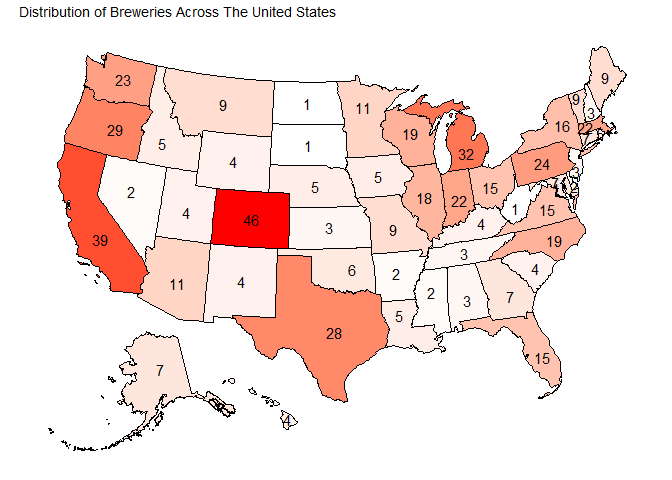
\includegraphics{ProjectMarkdown_files/figure-latex/unnamed-chunk-3-2.pdf}

\begin{Shaded}
\begin{Highlighting}[]
\CommentTok{\# table for display in RMD file}
\FunctionTok{kable}\NormalTok{(state\_num\_data }\SpecialCharTok{\%\textgreater{}\%} \FunctionTok{group\_by}\NormalTok{(State) }\SpecialCharTok{\%\textgreater{}\%}
\FunctionTok{summarise}\NormalTok{(}\AttributeTok{num\_brew =} \FunctionTok{n\_distinct}\NormalTok{(Brew\_name),}
\AttributeTok{mean\_abv =} \FunctionTok{mean}\NormalTok{(ABV), }\AttributeTok{mean\_ibu =} \FunctionTok{mean}\NormalTok{(IBU)) }\SpecialCharTok{\%\textgreater{}\%}
\FunctionTok{arrange}\NormalTok{(}\FunctionTok{desc}\NormalTok{(num\_brew)))}
\end{Highlighting}
\end{Shaded}

\begin{longtable}[]{@{}lrrr@{}}
\toprule()
State & num\_brew & mean\_abv & mean\_ibu \\
\midrule()
\endhead
CO & 46 & NA & NA \\
CA & 39 & 0.0599231 & NA \\
MI & 32 & NA & NA \\
OR & 29 & 0.0568276 & NA \\
TX & 28 & NA & NA \\
PA & 24 & NA & NA \\
WA & 23 & 0.0584348 & NA \\
IN & 22 & 0.0608182 & NA \\
MA & 22 & 0.0575455 & NA \\
NC & 19 & NA & NA \\
WI & 19 & 0.0522632 & NA \\
IL & 18 & 0.0581111 & NA \\
NY & 16 & NA & NA \\
FL & 15 & NA & NA \\
OH & 15 & 0.0661333 & NA \\
VA & 15 & 0.0593333 & NA \\
AZ & 11 & NA & NA \\
MN & 11 & 0.0630909 & NA \\
ME & 9 & 0.0570000 & NA \\
MO & 9 & 0.0605556 & NA \\
MT & 9 & NA & NA \\
VT & 9 & 0.0563333 & NA \\
AK & 7 & 0.0522857 & NA \\
CT & 7 & 0.0581429 & NA \\
GA & 7 & 0.0532857 & NA \\
MD & 7 & 0.0578571 & NA \\
OK & 6 & 0.0580000 & NA \\
IA & 5 & 0.0574000 & NA \\
ID & 5 & 0.0636000 & NA \\
LA & 5 & 0.0580000 & NA \\
NE & 5 & NA & NA \\
RI & 5 & 0.0542000 & NA \\
HI & 4 & 0.0505000 & NA \\
KY & 4 & 0.0652500 & NA \\
NM & 4 & 0.0617500 & NA \\
SC & 4 & 0.0615000 & NA \\
UT & 4 & 0.0475000 & NA \\
WY & 4 & 0.0572500 & NA \\
AL & 3 & 0.0626667 & NA \\
KS & 3 & 0.0483333 & 28.66667 \\
NH & 3 & 0.0460000 & NA \\
NJ & 3 & 0.0510000 & 43.33333 \\
TN & 3 & 0.0500000 & 30.66667 \\
AR & 2 & 0.0485000 & NA \\
DE & 2 & NA & NA \\
MS & 2 & 0.0575000 & 41.50000 \\
NV & 2 & NA & NA \\
DC & 1 & 0.0500000 & 15.00000 \\
ND & 1 & 0.0500000 & 32.00000 \\
SD & 1 & 0.0550000 & NA \\
WV & 1 & 0.0670000 & 71.00000 \\
\bottomrule()
\end{longtable}

\hypertarget{question-of-interest-3}{%
\subsection{Question of interest 3:}\label{question-of-interest-3}}

\hypertarget{address-the-missing-values}{%
\paragraph{Address The Missing
Values}\label{address-the-missing-values}}

Upon working with the data we found a number of missing values. While we
were able to remedy most of the issues found, the ones mentioned below
are data that either were not relevant to the data set, or were left out
because of different reporting mechanisms or the absence of a
requirement to report.

\begin{itemize}
\item
  CAN'd Aid: Oskar Blues Brewery teamed up with CAN'd Aid Foundation to
  fill cans of drinking water for residents in Southeast Texas. The
  missing value can be attributed to this item not having a style of
  alcohol since it is water which is not a form of alcohol.
\item
  Crowler: CROWLER (CAN + growler) is a 32-ounce or 25-ounce CAN filled
  with fresh craft beer from the draft source. The missing values here
  are attributed to this not being an actual drink.
\item
  Special Release: This beer was shown through various searches to be a
  retired drink. Because of it's retired status there didn't seem to be
  any information of relevance.
\item
  IBU \& ABV (Explicit Values): The IBU and ABV columns list almost half
  of their values as ``NA''. It would be unwise to remove this data
  since it would misrepresent the presence of breweries and their
  offerings. Imputing the values of this data was under consideration
  but given that the variability of the values differs on markets,
  breweries, and crafting styles it did not seem like an effective
  method for resolving these missing values.
\end{itemize}

\hypertarget{question-of-interest-4}{%
\subsection{Question of Interest 4:}\label{question-of-interest-4}}

\hypertarget{investigate-the-median-value-of-alcohol-content-and-international-bitterness-unit-for-each-state.}{%
\paragraph{Investigate the Median Value of Alcohol Content and
International Bitterness Unit for each
state.}\label{investigate-the-median-value-of-alcohol-content-and-international-bitterness-unit-for-each-state.}}

The median values of Alcohol content and International Bitterness Units
are displayed in the tables below. It is worth mentioning that the
missing ABV and IBU values effect the presence of breweries on the map.
This change in visualization is due to the missing values not being
included in the median calculations which effects the representation of
that data on the map. A specific example of this would be the removal
(grayed out portion) of South Dakota when visualizing the results for
the median IBU.

\begin{Shaded}
\begin{Highlighting}[]
\DocumentationTok{\#\#\#\#\#\#\#\#\#\#\#\#\#\#\#\#\#\#\#\#\#\#\#\#\#\#\#\#\#\#\#\#\#\#\# Question 4 \#\#\#\#\#\#\#\#\#\#\#\#\#\#\#\#\#\#\#\#\#\#\#\#\#\#\#\#\#\#\#\#\#\#}

\CommentTok{\# this will return medians for each state ( NA NOT INCLUDED )}
\NormalTok{state\_medians }\OtherTok{\textless{}{-}}\NormalTok{ beer\_brew }\SpecialCharTok{\%\textgreater{}\%} \FunctionTok{group\_by}\NormalTok{(State) }\SpecialCharTok{\%\textgreater{}\%}
  \FunctionTok{summarise}\NormalTok{(}\AttributeTok{num\_brew =} \FunctionTok{n\_distinct}\NormalTok{(Brew\_name),}
            \AttributeTok{median\_abv =} \FunctionTok{median}\NormalTok{(ABV, }\AttributeTok{na.rm =} \ConstantTok{TRUE}\NormalTok{), }\AttributeTok{median\_ibu =} \FunctionTok{median}\NormalTok{(IBU, }\AttributeTok{na.rm =} \ConstantTok{TRUE}\NormalTok{)) }\SpecialCharTok{\%\textgreater{}\%}
  \FunctionTok{arrange}\NormalTok{(}\FunctionTok{desc}\NormalTok{(num\_brew))}

\CommentTok{\# to return the medians data}
\CommentTok{\# state\_medians}

\CommentTok{\# convert to data frame}
\NormalTok{state\_medians }\OtherTok{\textless{}{-}} \FunctionTok{as.data.frame}\NormalTok{(state\_medians)}

\CommentTok{\# convert variable column from S to s (upper to lower) so that it works with data in next question}
\FunctionTok{names}\NormalTok{(state\_medians)[}\DecValTok{1}\NormalTok{] }\OtherTok{\textless{}{-}} \StringTok{\textquotesingle{}state\textquotesingle{}}

\CommentTok{\# plot Median ABV}
\NormalTok{state\_medians }\SpecialCharTok{\%\textgreater{}\%} \FunctionTok{ggplot}\NormalTok{(}\FunctionTok{aes}\NormalTok{(}\AttributeTok{x =} \FunctionTok{reorder}\NormalTok{(state, }\FunctionTok{desc}\NormalTok{(median\_abv)), }\AttributeTok{y =}\NormalTok{ median\_abv}\SpecialCharTok{*}\DecValTok{100}\NormalTok{, }\AttributeTok{fill =}\NormalTok{ state))}\SpecialCharTok{+}
  \FunctionTok{geom\_bar}\NormalTok{(}\AttributeTok{stat=}\StringTok{\textquotesingle{}identity\textquotesingle{}}\NormalTok{, }\AttributeTok{show.legend =} \ConstantTok{FALSE}\NormalTok{)}\SpecialCharTok{+}
  \FunctionTok{coord\_flip}\NormalTok{() }\SpecialCharTok{+}
  \FunctionTok{ggtitle}\NormalTok{(}\StringTok{"Bar Plot of Median Alcohol by Volume (ABV) Values for each State"}\NormalTok{) }\SpecialCharTok{+}
  \FunctionTok{xlab}\NormalTok{(}\StringTok{"State by Abbreviation"}\NormalTok{)}\SpecialCharTok{+}
  \FunctionTok{ylab}\NormalTok{(}\StringTok{"Median Value of Alcohol by Volume in Percent"}\NormalTok{)}
\end{Highlighting}
\end{Shaded}

\includegraphics{ProjectMarkdown_files/figure-latex/unnamed-chunk-4-1.pdf}

\begin{Shaded}
\begin{Highlighting}[]
\CommentTok{\# plot Median IBU}
\NormalTok{state\_medians }\SpecialCharTok{\%\textgreater{}\%} \FunctionTok{ggplot}\NormalTok{(}\FunctionTok{aes}\NormalTok{(}\AttributeTok{x =} \FunctionTok{reorder}\NormalTok{(state, }\FunctionTok{desc}\NormalTok{(median\_ibu)), }\AttributeTok{y =}\NormalTok{ median\_ibu, }\AttributeTok{fill =}\NormalTok{ state))}\SpecialCharTok{+}
  \FunctionTok{geom\_bar}\NormalTok{(}\AttributeTok{stat =} \StringTok{\textquotesingle{}identity\textquotesingle{}}\NormalTok{, }\AttributeTok{show.legend =} \ConstantTok{FALSE}\NormalTok{) }\SpecialCharTok{+}
  \FunctionTok{coord\_flip}\NormalTok{() }\SpecialCharTok{+}
  \FunctionTok{ggtitle}\NormalTok{(}\StringTok{"Bar plot of Median IBU Values for each State"}\NormalTok{)}\SpecialCharTok{+}
  \FunctionTok{xlab}\NormalTok{(}\StringTok{"State by Abbreviation"}\NormalTok{)}\SpecialCharTok{+}
  \FunctionTok{ylab}\NormalTok{(}\StringTok{"Median International Bitterness Units (IBU)"}\NormalTok{)}
\end{Highlighting}
\end{Shaded}

\includegraphics{ProjectMarkdown_files/figure-latex/unnamed-chunk-4-2.pdf}

\begin{Shaded}
\begin{Highlighting}[]
\CommentTok{\# creating a variable to call for median labels}
\NormalTok{median\_labels }\OtherTok{\textless{}{-}} \FunctionTok{merge}\NormalTok{(centroid\_labels, state\_medians, }\AttributeTok{by =}\StringTok{\textquotesingle{}state\textquotesingle{}}\NormalTok{)}

\CommentTok{\# create the ABV map}
\NormalTok{abv\_state\_plot }\OtherTok{\textless{}{-}} \FunctionTok{plot\_usmap}\NormalTok{(}\AttributeTok{data =}\NormalTok{ state\_medians[,}\DecValTok{1}\SpecialCharTok{:}\DecValTok{3}\NormalTok{],}
                             \AttributeTok{values =} \StringTok{"median\_abv"}\NormalTok{,}
                             \AttributeTok{color =} \StringTok{"black"}\NormalTok{,}
                             \AttributeTok{labels =}\NormalTok{ F) }\SpecialCharTok{+}
  \FunctionTok{guides}\NormalTok{(}\AttributeTok{fill =} \StringTok{"none"}\NormalTok{) }\SpecialCharTok{+}
  \FunctionTok{geom\_text}\NormalTok{(}\AttributeTok{data =}\NormalTok{ median\_labels, }\FunctionTok{aes}\NormalTok{(}
    \AttributeTok{x =}\NormalTok{ x, }\AttributeTok{y =}\NormalTok{ y,}
    \AttributeTok{label =}\NormalTok{ scales}\SpecialCharTok{::}\FunctionTok{number}\NormalTok{(median\_abv }\SpecialCharTok{*} \DecValTok{100}\NormalTok{, }\AttributeTok{accuracy =} \FloatTok{0.01}\NormalTok{)), }\AttributeTok{color =} \StringTok{"black"}\NormalTok{) }\SpecialCharTok{+}
  \FunctionTok{scale\_fill\_gradient}\NormalTok{(}\AttributeTok{low =} \StringTok{"white"}\NormalTok{, }\AttributeTok{high =} \StringTok{"red"}\NormalTok{) }\SpecialCharTok{+}
  \FunctionTok{labs}\NormalTok{(}\AttributeTok{title =} \StringTok{"Distribution of Median ABV per State"}\NormalTok{)}

\CommentTok{\# create the IBU map}
\NormalTok{ibu\_state\_plot }\OtherTok{\textless{}{-}} \FunctionTok{plot\_usmap}\NormalTok{(}\AttributeTok{data =}\NormalTok{ state\_medians[,}\DecValTok{1}\SpecialCharTok{:}\DecValTok{4}\NormalTok{],}
                             \AttributeTok{values =} \StringTok{"median\_ibu"}\NormalTok{,}
                             \AttributeTok{color =} \StringTok{"black"}\NormalTok{,}
                             \AttributeTok{labels =}\NormalTok{ F)}\SpecialCharTok{+}
  \FunctionTok{guides}\NormalTok{(}\AttributeTok{fill =} \StringTok{"none"}\NormalTok{)}\SpecialCharTok{+}
  \FunctionTok{geom\_text}\NormalTok{(}\AttributeTok{data =}\NormalTok{ median\_labels, }\FunctionTok{aes}\NormalTok{(}
    \AttributeTok{x =}\NormalTok{ x, }\AttributeTok{y =}\NormalTok{ y,}
    \AttributeTok{label =}\NormalTok{ scales}\SpecialCharTok{::}\FunctionTok{number}\NormalTok{(median\_ibu, }\AttributeTok{accuracy =} \DecValTok{1}\NormalTok{)), }\AttributeTok{color =} \StringTok{"black"}\NormalTok{) }\SpecialCharTok{+}
  \FunctionTok{scale\_fill\_gradient}\NormalTok{(}\AttributeTok{low =} \StringTok{"white"}\NormalTok{, }\AttributeTok{high =} \StringTok{"red"}\NormalTok{)}\SpecialCharTok{+}
  \FunctionTok{labs}\NormalTok{(}\AttributeTok{title =} \StringTok{"Distribution of Median IBU per State"}\NormalTok{)}

\CommentTok{\# plot the ABV Median state plot}
\NormalTok{abv\_state\_plot}
\end{Highlighting}
\end{Shaded}

\includegraphics{ProjectMarkdown_files/figure-latex/unnamed-chunk-4-3.pdf}

\begin{Shaded}
\begin{Highlighting}[]
\CommentTok{\# plot the IBU Median state plot}
\NormalTok{ibu\_state\_plot}
\end{Highlighting}
\end{Shaded}

\includegraphics{ProjectMarkdown_files/figure-latex/unnamed-chunk-4-4.pdf}

\hypertarget{question-of-interest-5}{%
\subsection{Question of Interest 5:}\label{question-of-interest-5}}

\hypertarget{determine-which-states-contain-the-highest-value-of-alcohol-by-volume-abv-and-international-bitterness-units-ibu.}{%
\paragraph{Determine Which States Contain the Highest Value of Alcohol
by Volume (ABV) and International Bitterness Units
(IBU).}\label{determine-which-states-contain-the-highest-value-of-alcohol-by-volume-abv-and-international-bitterness-units-ibu.}}

The State with the highest Alcohol by Volume is Colorado (CO) at 12.8\%.
This was determined by selecting only the State and IBU columns then
running a function which would interpret the Max value.

The State with the highest International Bitterness Unit is Oregon (OR)
at 138 IBUs. This value was determined by selecting only the State and
IBU columns then running a function which would interpret the Max value.

\begin{Shaded}
\begin{Highlighting}[]
\DocumentationTok{\#\#\#\#\#\#\#\#\#\#\#\#\#\#\#\#\#\#\#\#\#\#\#\#\#\#\#\#\#\#\#\#\#\#\# Question 5 \#\#\#\#\#\#\#\#\#\#\#\#\#\#\#\#\#\#\#\#\#\#\#\#\#\#\#\#\#\#\#\#\#\#}

\CommentTok{\# to call on selected data that will only return the sought after information}
\NormalTok{max\_abv }\OtherTok{\textless{}{-}}\NormalTok{ beer\_brew }\SpecialCharTok{\%\textgreater{}\%} \FunctionTok{select}\NormalTok{(ABV, State)}

\NormalTok{max\_abv[}\FunctionTok{which.max}\NormalTok{(max\_abv}\SpecialCharTok{$}\NormalTok{ABV),]}
\end{Highlighting}
\end{Shaded}

\begin{verbatim}
      ABV State
369 0.128    CO
\end{verbatim}

\begin{Shaded}
\begin{Highlighting}[]
\CommentTok{\# mean(max\_abv$ABV, na.rm = TRUE) * 100 \# 5.99 \%}
\CommentTok{\# median(max\_abv$ABV, na.rm = TRUE) * 100 \# 5.7 \%}
\CommentTok{\# plot for IBU}
\NormalTok{max\_ibu }\OtherTok{\textless{}{-}}\NormalTok{ beer\_brew }\SpecialCharTok{\%\textgreater{}\%} \FunctionTok{select}\NormalTok{(IBU, State)}

\NormalTok{max\_ibu[}\FunctionTok{which.max}\NormalTok{(max\_ibu}\SpecialCharTok{$}\NormalTok{IBU),]}
\end{Highlighting}
\end{Shaded}

\begin{verbatim}
     IBU State
1771 138    OR
\end{verbatim}

\begin{Shaded}
\begin{Highlighting}[]
\CommentTok{\# mean(max\_ibu$IBU, na.rm = TRUE) \# 42.955}
\CommentTok{\# median(max\_ibu$IBU, na.rm = TRUE) \# 35}
\end{Highlighting}
\end{Shaded}

\hypertarget{question-of-interest-6}{%
\subsection{Question of Interest 6:}\label{question-of-interest-6}}

\hypertarget{comment-on-the-summary-statistics-distribution-of-the-alcohol-by-volume-abv-variable}{%
\paragraph{Comment on the Summary Statistics \& Distribution of The
Alcohol by Volume (ABV)
Variable}\label{comment-on-the-summary-statistics-distribution-of-the-alcohol-by-volume-abv-variable}}

The Distribution of Alcohol by Volume across the United States appears
to have a right skew to the data. This right skew can be interpreted as
a distribution of data in which there tends to be a higher instance of
larger values to the right of the median in the data, as opposed to an
equal portion of large and small values to the right and left of the
mean. A visual representation of this can be viewed below.

\begin{Shaded}
\begin{Highlighting}[]
\DocumentationTok{\#\#\#\#\#\#\#\#\#\#\#\#\#\#\#\#\#\#\#\#\#\#\#\#\#\#\#\#\#\#\#\#\#\#\# Question 6 \#\#\#\#\#\#\#\#\#\#\#\#\#\#\#\#\#\#\#\#\#\#\#\#\#\#\#\#\#\#\#\#\#\#}

\NormalTok{abv\_dis\_plot }\OtherTok{\textless{}{-}}\NormalTok{ beer\_brew }\SpecialCharTok{\%\textgreater{}\%} \FunctionTok{select}\NormalTok{(ABV,Brewery\_id)}
\NormalTok{abv\_dis\_plot }\SpecialCharTok{\%\textgreater{}\%} \FunctionTok{ggplot}\NormalTok{(}\FunctionTok{aes}\NormalTok{(ABV }\SpecialCharTok{*} \DecValTok{100}\NormalTok{)) }\SpecialCharTok{+}
  \FunctionTok{geom\_histogram}\NormalTok{(}\AttributeTok{color =} \StringTok{\textquotesingle{}black\textquotesingle{}}\NormalTok{,}\FunctionTok{aes}\NormalTok{(}\AttributeTok{fill =} \StringTok{\textquotesingle{}red\textquotesingle{}}\NormalTok{), }\AttributeTok{binwidth =}\NormalTok{ .}\DecValTok{25}\NormalTok{, }\AttributeTok{alpha =}\NormalTok{ .}\DecValTok{5}\NormalTok{, }\AttributeTok{show.legend =} \ConstantTok{FALSE}\NormalTok{) }\SpecialCharTok{+}
  \FunctionTok{ggtitle}\NormalTok{(}\StringTok{\textquotesingle{}Distribution of the Alcohol by Volume Content in Beer From Various Breweries\textquotesingle{}}\NormalTok{)}\SpecialCharTok{+}
  \FunctionTok{ylab}\NormalTok{(}\StringTok{\textquotesingle{}Frequency\textquotesingle{}}\NormalTok{) }\SpecialCharTok{+} \FunctionTok{xlab}\NormalTok{(}\StringTok{\textquotesingle{}Alcohol by Volume in Percent \%\textquotesingle{}}\NormalTok{)}
\end{Highlighting}
\end{Shaded}

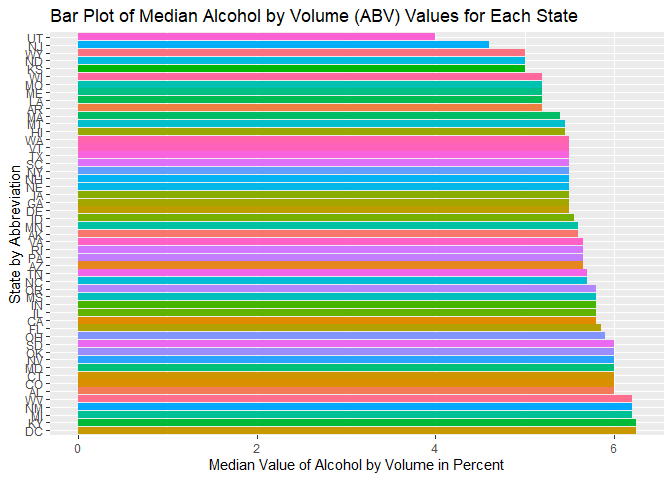
\includegraphics{ProjectMarkdown_files/figure-latex/unnamed-chunk-6-1.pdf}

\begin{Shaded}
\begin{Highlighting}[]
\FunctionTok{summary}\NormalTok{(beer\_brew}\SpecialCharTok{$}\NormalTok{ABV }\SpecialCharTok{*} \DecValTok{100}\NormalTok{)}
\end{Highlighting}
\end{Shaded}

\begin{verbatim}
   Min. 1st Qu.  Median    Mean 3rd Qu.    Max.    NA's 
  0.100   5.000   5.700   5.993   6.800  12.800      60 
\end{verbatim}

\hypertarget{question-of-interest-7}{%
\subsection{Question of Interest 7:}\label{question-of-interest-7}}

\hypertarget{is-there-an-apparent-relationship-between-the-bitterness-of-the-beer-and-its-alcoholic-content}{%
\paragraph{Is there an apparent relationship between the bitterness of
the beer and its alcoholic
content?}\label{is-there-an-apparent-relationship-between-the-bitterness-of-the-beer-and-its-alcoholic-content}}

It appears that there is a positive relationship between the bitterness
of beer and its alcoholic content. We can visualize on a scatter plot
that as the bitterness rating increases there tends to be an increase in
Alcohol by Volume Percentage (ABV).

We created a series of scatter plots that would help clean up the
visualization of the relationship between IBU and ABV as they relate to
different styles. These plots are below:

\hypertarget{first-this-plot-shows-us-the-general-relationship-with-all-styles-included.}{%
\subsubsection{1. First this plot shows us the general relationship with
all styles
included.}\label{first-this-plot-shows-us-the-general-relationship-with-all-styles-included.}}

\begin{Shaded}
\begin{Highlighting}[]
\DocumentationTok{\#\#\#\#\#\#\#\#\#\#\#\#\#\#\#\#\#\#\#\#\#\#\#\#\#\#\#\#\#\#\#\#\#\#\# Question 7 \#\#\#\#\#\#\#\#\#\#\#\#\#\#\#\#\#\#\#\#\#\#\#\#\#\#\#\#\#\#\#\#\#\#}

\NormalTok{ibu\_abv\_plot }\OtherTok{\textless{}{-}}\NormalTok{ beer\_brew }\SpecialCharTok{\%\textgreater{}\%} \FunctionTok{select}\NormalTok{(IBU,ABV,Style)}
             
\NormalTok{ibu\_abv\_plot }\SpecialCharTok{\%\textgreater{}\%} \FunctionTok{ggplot}\NormalTok{(}\FunctionTok{aes}\NormalTok{(}\AttributeTok{x =}\NormalTok{ ABV, }\AttributeTok{y =}\NormalTok{ IBU)) }\SpecialCharTok{+} 
  \FunctionTok{geom\_point}\NormalTok{(}\FunctionTok{aes}\NormalTok{(}\AttributeTok{color =}\NormalTok{ Style), }\AttributeTok{show.legend =} \ConstantTok{FALSE}\NormalTok{) }\SpecialCharTok{+} 
  \FunctionTok{geom\_smooth}\NormalTok{(}\AttributeTok{se =} \ConstantTok{FALSE}\NormalTok{, }\AttributeTok{color =} \StringTok{"black"}\NormalTok{) }\SpecialCharTok{+}
  \FunctionTok{ggtitle}\NormalTok{(}\StringTok{"Scatterplot of ABV and IBU Values of All Beer Styles"}\NormalTok{)}\SpecialCharTok{+}\FunctionTok{xlab}\NormalTok{(}\StringTok{"Alcohol by Volume in Percent \%"}\NormalTok{)}\SpecialCharTok{+}\FunctionTok{ylab}\NormalTok{(}\StringTok{"Bitterness Rating (IBUs)"}\NormalTok{)}
\end{Highlighting}
\end{Shaded}

\begin{verbatim}
## `geom_smooth()` using method = 'gam' and formula 'y ~ s(x, bs = "cs")'
\end{verbatim}

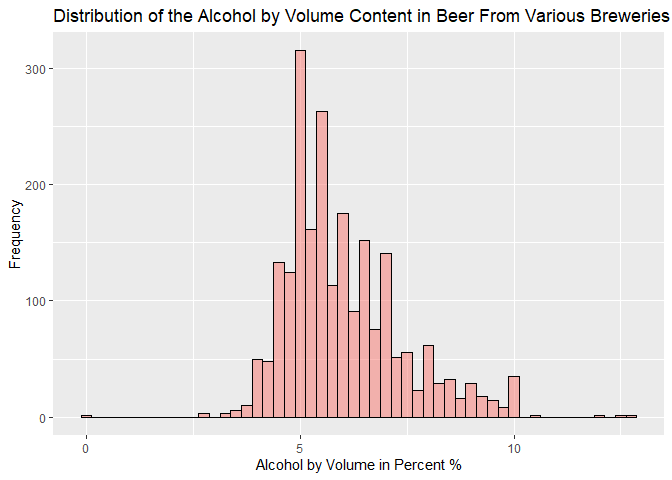
\includegraphics{ProjectMarkdown_files/figure-latex/unnamed-chunk-8-1.pdf}

\hypertarget{this-visualization-is-the-same-but-filtered-for-only-ipa-beverages.}{%
\subsubsection{2. This visualization is the same but filtered for only
IPA
beverages.}\label{this-visualization-is-the-same-but-filtered-for-only-ipa-beverages.}}

\begin{Shaded}
\begin{Highlighting}[]
\CommentTok{\# visualizing scatter plot of ABV and IBU with Style filter for all IPA }
\NormalTok{ipa\_viz }\OtherTok{\textless{}{-}}\NormalTok{ ibu\_abv\_plot }\SpecialCharTok{\%\textgreater{}\%} \FunctionTok{filter}\NormalTok{(}\FunctionTok{str\_detect}\NormalTok{(Style, }\StringTok{\textquotesingle{}IPA\textquotesingle{}}\NormalTok{))}

\NormalTok{ipa\_viz }\SpecialCharTok{\%\textgreater{}\%} \FunctionTok{ggplot}\NormalTok{(}\FunctionTok{aes}\NormalTok{(}\AttributeTok{x =}\NormalTok{ ABV, }\AttributeTok{y =}\NormalTok{ IBU)) }\SpecialCharTok{+}
  \FunctionTok{geom\_point}\NormalTok{(}\FunctionTok{aes}\NormalTok{(}\AttributeTok{color =}\NormalTok{ Style))}\SpecialCharTok{+}
  \FunctionTok{geom\_smooth}\NormalTok{(}\AttributeTok{se =} \ConstantTok{FALSE}\NormalTok{, }\AttributeTok{color =} \StringTok{\textquotesingle{}black\textquotesingle{}}\NormalTok{) }\SpecialCharTok{+}
  \FunctionTok{ggtitle}\NormalTok{(}\StringTok{"Scatterplot of ABV and IBU Values of Only IPA Beer Style"}\NormalTok{)}\SpecialCharTok{+}\FunctionTok{xlab}\NormalTok{(}\StringTok{"Alcohol by Volume in Percent \%"}\NormalTok{)}\SpecialCharTok{+}\FunctionTok{ylab}\NormalTok{(}\StringTok{"Bitterness Rating (IBUs)"}\NormalTok{)}
\end{Highlighting}
\end{Shaded}

\begin{verbatim}
## `geom_smooth()` using method = 'loess' and formula 'y ~ x'
\end{verbatim}

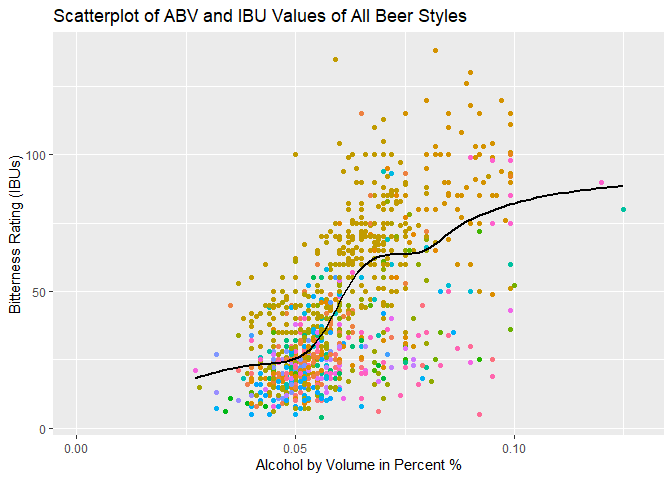
\includegraphics{ProjectMarkdown_files/figure-latex/unnamed-chunk-9-1.pdf}

\hypertarget{below-you-will-see-a-scatter-plot-filtered-to-visualize-the-same-abv-ibu-relationship-with-only-ale-beverages.}{%
\subsubsection{3. Below you will see a scatter plot filtered to
visualize the same ABV, IBU relationship with only Ale
beverages.}\label{below-you-will-see-a-scatter-plot-filtered-to-visualize-the-same-abv-ibu-relationship-with-only-ale-beverages.}}

\begin{Shaded}
\begin{Highlighting}[]
\CommentTok{\# visualizing scatter plot of ABV and IBU with Style filter for all ALE}
\NormalTok{ale\_viz }\OtherTok{\textless{}{-}}\NormalTok{ ibu\_abv\_plot }\SpecialCharTok{\%\textgreater{}\%} \FunctionTok{filter}\NormalTok{(}\FunctionTok{str\_detect}\NormalTok{(Style, }\StringTok{"Ale"}\NormalTok{))}

\NormalTok{ale\_viz }\SpecialCharTok{\%\textgreater{}\%} \FunctionTok{ggplot}\NormalTok{(}\FunctionTok{aes}\NormalTok{(}\AttributeTok{x =}\NormalTok{ ABV, }\AttributeTok{y =}\NormalTok{ IBU)) }\SpecialCharTok{+}
  \FunctionTok{geom\_point}\NormalTok{(}\FunctionTok{aes}\NormalTok{( }\AttributeTok{color =}\NormalTok{ Style), }\AttributeTok{show.legend =} \ConstantTok{FALSE}\NormalTok{) }\SpecialCharTok{+}
  \FunctionTok{geom\_smooth}\NormalTok{(}\AttributeTok{se =} \ConstantTok{FALSE}\NormalTok{, }\AttributeTok{color =} \StringTok{\textquotesingle{}black\textquotesingle{}}\NormalTok{) }\SpecialCharTok{+}
  \FunctionTok{ggtitle}\NormalTok{(}\StringTok{"Scatterplot of ABV and IBU Values of Only Ale Beer Style"}\NormalTok{)}\SpecialCharTok{+}\FunctionTok{xlab}\NormalTok{(}\StringTok{"Alcohol by Volume in Percent \%"}\NormalTok{)}\SpecialCharTok{+}\FunctionTok{ylab}\NormalTok{(}\StringTok{"Bitterness Rating (IBUs)"}\NormalTok{)}
\end{Highlighting}
\end{Shaded}

\begin{verbatim}
## `geom_smooth()` using method = 'loess' and formula 'y ~ x'
\end{verbatim}

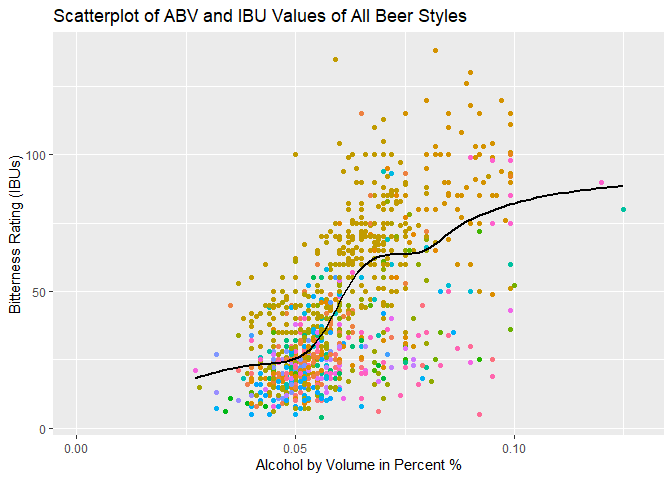
\includegraphics{ProjectMarkdown_files/figure-latex/unnamed-chunk-10-1.pdf}

\hypertarget{finally-this-scatter-plot-displays-the-abv-ibu-relationship-with-styles-filterd-to-include-every-type-that-is-not-ipa-or-ale.}{%
\subsubsection{4. Finally this scatter plot displays the ABV, IBU
relationship with styles filterd to include every type that is NOT IPA,
or
Ale.}\label{finally-this-scatter-plot-displays-the-abv-ibu-relationship-with-styles-filterd-to-include-every-type-that-is-not-ipa-or-ale.}}

\begin{Shaded}
\begin{Highlighting}[]
\CommentTok{\# visualizing scatter plot of ABV and IBU with style filter for not ALE, or IPA}
\NormalTok{else\_viz }\OtherTok{\textless{}{-}}\NormalTok{ ibu\_abv\_plot }\SpecialCharTok{\%\textgreater{}\%} \FunctionTok{filter}\NormalTok{(}\SpecialCharTok{!}\FunctionTok{str\_detect}\NormalTok{(Style, }\StringTok{"Ale"}\NormalTok{)) }\SpecialCharTok{\%\textgreater{}\%} \FunctionTok{filter}\NormalTok{(}\SpecialCharTok{!}\FunctionTok{str\_detect}\NormalTok{(Style, }\StringTok{"IPA"}\NormalTok{))}

\NormalTok{else\_viz }\SpecialCharTok{\%\textgreater{}\%} \FunctionTok{ggplot}\NormalTok{(}\FunctionTok{aes}\NormalTok{(}\AttributeTok{x =}\NormalTok{ ABV }\SpecialCharTok{*} \DecValTok{100}\NormalTok{, }\AttributeTok{y =}\NormalTok{ IBU)) }\SpecialCharTok{+}
  \FunctionTok{geom\_point}\NormalTok{(}\FunctionTok{aes}\NormalTok{(}\AttributeTok{color =}\NormalTok{ Style), }\AttributeTok{show.legend =} \ConstantTok{FALSE}\NormalTok{) }\SpecialCharTok{+}
  \FunctionTok{geom\_smooth}\NormalTok{(}\AttributeTok{se =} \ConstantTok{FALSE}\NormalTok{, }\AttributeTok{color =} \StringTok{"black"}\NormalTok{) }\SpecialCharTok{+} 
  \FunctionTok{ggtitle}\NormalTok{(}\StringTok{"Scatterplot of ABV and IBU Values of Beer Styles Other than Ale, or IPA"}\NormalTok{) }\SpecialCharTok{+} \FunctionTok{xlab}\NormalTok{(}\StringTok{"Alcohol by Volume in Percent \%"}\NormalTok{)}\SpecialCharTok{+}\FunctionTok{ylab}\NormalTok{(}\StringTok{"Bitterness Rating (IBUs)"}\NormalTok{)}
\end{Highlighting}
\end{Shaded}

\begin{verbatim}
## `geom_smooth()` using method = 'loess' and formula 'y ~ x'
\end{verbatim}

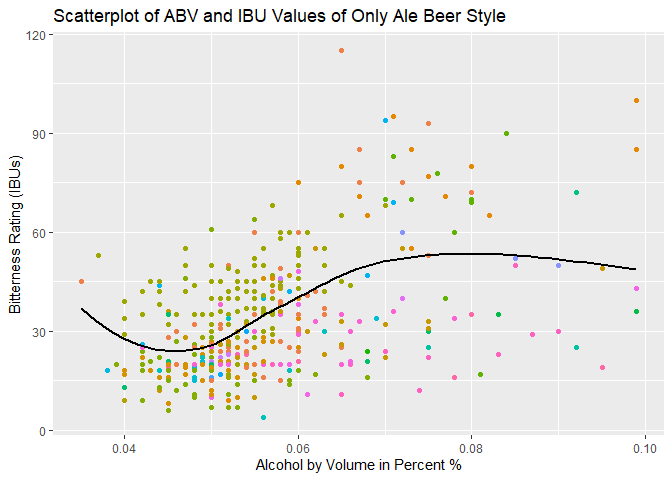
\includegraphics{ProjectMarkdown_files/figure-latex/unnamed-chunk-11-1.pdf}

\hypertarget{it-appears-that-across-most-styles-of-beer-there-is-a-positive-relationship-between-ibu-and-abv.-it-is-worth-discussing-however-the-ale-style-of-beer-has-somewhat-of-a-curved-arguably-non-linear-relationship.-the-majority-of-values-in-which-abv-is-greater-than-6-appear-to-be-of-an-equal-distribution-about-the-y-axis-and-lose-their-visual-power-to-explain-the-variance-of-ibu-ratings.}{%
\paragraph{It appears that across most styles of beer there is a
positive relationship between IBU and ABV. It is worth discussing
however the ``Ale'' style of beer has somewhat of a curved arguably
non-linear relationship. The majority of values in which ABV is greater
than 6\% appear to be of an equal distribution about the y-axis, and
lose their visual power to explain the variance of IBU
ratings.}\label{it-appears-that-across-most-styles-of-beer-there-is-a-positive-relationship-between-ibu-and-abv.-it-is-worth-discussing-however-the-ale-style-of-beer-has-somewhat-of-a-curved-arguably-non-linear-relationship.-the-majority-of-values-in-which-abv-is-greater-than-6-appear-to-be-of-an-equal-distribution-about-the-y-axis-and-lose-their-visual-power-to-explain-the-variance-of-ibu-ratings.}}

\hypertarget{question-of-interest-8}{%
\subsection{Question of Interest 8:}\label{question-of-interest-8}}

\hypertarget{investigate-the-difference-with-respect-to-ibu-and-abv-between-ipas-and-other-types-of-ale.}{%
\paragraph{Investigate the difference with respect to IBU and ABV
between IPAs and other types of
Ale.}\label{investigate-the-difference-with-respect-to-ibu-and-abv-between-ipas-and-other-types-of-ale.}}

\begin{Shaded}
\begin{Highlighting}[]
\DocumentationTok{\#\#\#\#\#\#\#\#\#\#\#\#\#\#\#\#\#\#\#\#\#\#\#\#\#\#\#\#\#\#\#\#\#\#\# KNN Prediction Model Data \#\#\#\#\#\#\#\#\#\#\#\#\#\#\#\#\#\#\#\#\#\#\#\#\#}

\CommentTok{\# test to see how the model will work using beer\_brew}

\CommentTok{\# make a Dataframe without NA so that we can run KNN:}
\NormalTok{beer\_predict }\OtherTok{\textless{}{-}} \FunctionTok{na.omit}\NormalTok{(beer\_brew)}
\CommentTok{\# sanity check }
\CommentTok{\#view(beer\_predict)}

\CommentTok{\# creating a data frame that can be used to minimize the noise between Ale and IPA}
\NormalTok{ipa\_knn }\OtherTok{\textless{}{-}}\NormalTok{ beer\_predict }\SpecialCharTok{\%\textgreater{}\%} \FunctionTok{select}\NormalTok{(Brewery\_id,beer\_name, IBU, ABV, Style) }\SpecialCharTok{\%\textgreater{}\%}
  \FunctionTok{group\_by}\NormalTok{(Brewery\_id) }\SpecialCharTok{\%\textgreater{}\%} \FunctionTok{filter}\NormalTok{(}\FunctionTok{str\_detect}\NormalTok{(Style, }\StringTok{"IPA"}\NormalTok{)) }\SpecialCharTok{\%\textgreater{}\%}
  \FunctionTok{mutate}\NormalTok{(}\AttributeTok{Style =} \StringTok{"ipa"}\NormalTok{)}

\NormalTok{ale\_knn }\OtherTok{\textless{}{-}}\NormalTok{ beer\_predict }\SpecialCharTok{\%\textgreater{}\%} \FunctionTok{select}\NormalTok{(Brewery\_id,beer\_name, IBU, ABV, Style) }\SpecialCharTok{\%\textgreater{}\%}
  \FunctionTok{group\_by}\NormalTok{(Brewery\_id) }\SpecialCharTok{\%\textgreater{}\%} \FunctionTok{filter}\NormalTok{(}\FunctionTok{str\_detect}\NormalTok{(Style, }\StringTok{"Ale"}\NormalTok{)) }\SpecialCharTok{\%\textgreater{}\%} 
  \FunctionTok{mutate}\NormalTok{(}\AttributeTok{Style =} \StringTok{"ale"}\NormalTok{)}

\CommentTok{\# view(ipa\_knn)  \# 374}
\CommentTok{\# view(ale\_knn) \# 519}

\NormalTok{combine\_knn }\OtherTok{\textless{}{-}} \FunctionTok{full\_join}\NormalTok{(ipa\_knn, ale\_knn)}
\end{Highlighting}
\end{Shaded}

\begin{verbatim}
## Joining, by = c("Brewery_id", "beer_name", "IBU", "ABV", "Style")
\end{verbatim}

\begin{Shaded}
\begin{Highlighting}[]
\CommentTok{\# view(combine\_knn)}

\CommentTok{\# simple test to see if the data works together within the KNN function}
\CommentTok{\# my\_beer\_test \textless{}{-} data.frame(IBU = c(.05, .04, .043), ABV = c(.06, .055, .065))}
\CommentTok{\# knn(beer\_predict[,c(7,8)], my\_beer\_test, beer\_predict$Style, k = 3, prob = TRUE)}


\CommentTok{\# viewing what matches each of these strings will return before filtering. }
\CommentTok{\# (str\_view\_all(beer\_predict$Style, \textquotesingle{}Ale\textquotesingle{}, match = TRUE))}
\CommentTok{\# (str\_view\_all(beer\_predict$Style, \textquotesingle{}IPA\textquotesingle{}, match = TRUE))}

\CommentTok{\# creating test variable to call so we can see if the filter works}
\CommentTok{\#test\_ale\_filter \textless{}{-} beer\_predict \%\textgreater{}\% filter(str\_detect(Style, \textquotesingle{}Ale\textquotesingle{}))}
\CommentTok{\#view(test\_ale\_filter$Style) \# viewing the filter for effectiveness}

\CommentTok{\# repeating the same process for the IPA}
\CommentTok{\#test\_ipa\_filter \textless{}{-} beer\_predict \%\textgreater{}\% filter(str\_detect(Style, \textquotesingle{}IPA\textquotesingle{}))}
\CommentTok{\#view(test\_ipa\_filter$Style) \# viewing the filter for effectiveness }

\CommentTok{\# using both filters above to create one combo test filter}
\CommentTok{\#test\_combo\_filter\textless{}{-} beer\_predict \%\textgreater{}\% filter(str\_detect(Style, \textquotesingle{}IPA\textquotesingle{}) | str\_detect(Style, "Ale"))}
\CommentTok{\#view(test\_combo\_filter$Style)}


\CommentTok{\# creating the finalized data frame to use for test/train split etc. }
\CommentTok{\# beer\_predict\_fin \textless{}{-} beer\_predict \%\textgreater{}\% filter(str\_detect(Style, \textquotesingle{}IPA\textquotesingle{}) | str\_detect(Style, "Ale"))}
\CommentTok{\# glimpse(beer\_predict\_fin)}
\end{Highlighting}
\end{Shaded}

\begin{Shaded}
\begin{Highlighting}[]
\DocumentationTok{\#\#\#\#\#\#\#\#\#\#\#\#\#\#\#\#\#\#\#\#\#\#\#\#\#\#\#\#\#\#\#\#\#\#\# KNN Test type 2 \#\#\#\#\#\#\#\#\#\#\#\#\#\#\#\#\#\#\#\#\#\#\#\#\#}

\CommentTok{\#checking dimensions to understand what our test/train will look like}
\CommentTok{\# glimpse(beer\_predict\_fin)}
\CommentTok{\# nrow(combine\_knn) \# total 893 rows}
\CommentTok{\# round(nrow(combine\_knn)*.3) \# total 268}


\FunctionTok{set.seed}\NormalTok{(}\DecValTok{765}\NormalTok{)}
\NormalTok{intrain }\OtherTok{\textless{}{-}} \FunctionTok{sample}\NormalTok{(}\FunctionTok{nrow}\NormalTok{(combine\_knn), }\FunctionTok{round}\NormalTok{(}\FunctionTok{nrow}\NormalTok{(combine\_knn)}\SpecialCharTok{*}\NormalTok{.}\DecValTok{30}\NormalTok{))}
\NormalTok{beer\_train }\OtherTok{\textless{}{-}}\NormalTok{ combine\_knn[intrain,]}
\NormalTok{beer\_test }\OtherTok{\textless{}{-}}\NormalTok{ combine\_knn[}\SpecialCharTok{{-}}\NormalTok{intrain,]}


\CommentTok{\# setting up the classification }
\NormalTok{classification }\OtherTok{\textless{}{-}} \FunctionTok{knn}\NormalTok{(beer\_train[,}\FunctionTok{c}\NormalTok{(}\DecValTok{3}\NormalTok{,}\DecValTok{4}\NormalTok{)],}
\NormalTok{                      beer\_test[,}\FunctionTok{c}\NormalTok{(}\DecValTok{3}\NormalTok{,}\DecValTok{4}\NormalTok{)],}
\NormalTok{                      beer\_train}\SpecialCharTok{$}\NormalTok{Style,}
                      \AttributeTok{k =} \DecValTok{3}\NormalTok{, }\AttributeTok{prob =} \ConstantTok{TRUE}\NormalTok{)}

\CommentTok{\# setting up a passable data for confusion matrix }
\NormalTok{u }\OtherTok{\textless{}{-}} \FunctionTok{union}\NormalTok{(classification, beer\_test}\SpecialCharTok{$}\NormalTok{Style)}
\NormalTok{t }\OtherTok{\textless{}{-}} \FunctionTok{table}\NormalTok{(}\FunctionTok{factor}\NormalTok{(classification, u), }\FunctionTok{factor}\NormalTok{(beer\_test}\SpecialCharTok{$}\NormalTok{Style, u), }\AttributeTok{dnn =} \FunctionTok{c}\NormalTok{(}\StringTok{"Prediction"}\NormalTok{, }\StringTok{"Truth"}\NormalTok{))}

\CommentTok{\# confusion matrix for more stats on the model}
\NormalTok{CM }\OtherTok{\textless{}{-}} \FunctionTok{confusionMatrix}\NormalTok{(t)}

\NormalTok{beer\_knn\_plot }\OtherTok{\textless{}{-}} \FunctionTok{as.data.frame}\NormalTok{(CM}\SpecialCharTok{$}\NormalTok{table)}

\NormalTok{beer\_knn\_plot}\SpecialCharTok{$}\NormalTok{Prediction }\OtherTok{\textless{}{-}} \FunctionTok{factor}\NormalTok{(beer\_knn\_plot}\SpecialCharTok{$}\NormalTok{Prediction, }\AttributeTok{levels =} \FunctionTok{rev}\NormalTok{(}\FunctionTok{levels}\NormalTok{(beer\_knn\_plot}\SpecialCharTok{$}\NormalTok{Truth)))}

\FunctionTok{ggplot}\NormalTok{(beer\_knn\_plot, }\FunctionTok{aes}\NormalTok{(Prediction, Truth, }\AttributeTok{fill =}\NormalTok{ (Freq))) }\SpecialCharTok{+}
  \FunctionTok{geom\_tile}\NormalTok{(}\AttributeTok{show.legend =} \ConstantTok{FALSE}\NormalTok{) }\SpecialCharTok{+} \FunctionTok{geom\_text}\NormalTok{(}\FunctionTok{aes}\NormalTok{(}\AttributeTok{label =}\NormalTok{ (Freq))) }\SpecialCharTok{+}
  \FunctionTok{scale\_fill\_gradient}\NormalTok{(}\AttributeTok{low =} \StringTok{"light blue"}\NormalTok{, }\AttributeTok{high =} \StringTok{"\#009194"}\NormalTok{) }\SpecialCharTok{+}
  \FunctionTok{labs}\NormalTok{(}\AttributeTok{x =} \StringTok{"Truth"}\NormalTok{, }\AttributeTok{y =} \StringTok{"Prediction"}\NormalTok{) }\SpecialCharTok{+}
  \FunctionTok{scale\_x\_discrete}\NormalTok{(}\AttributeTok{labels =} \FunctionTok{c}\NormalTok{(}\StringTok{"IPA"}\NormalTok{, }\StringTok{"Ale"}\NormalTok{)) }\SpecialCharTok{+}
  \FunctionTok{scale\_y\_discrete}\NormalTok{(}\AttributeTok{labels =} \FunctionTok{c}\NormalTok{(}\StringTok{"Ale"}\NormalTok{, }\StringTok{"IPA"}\NormalTok{))}\SpecialCharTok{+}
  \FunctionTok{coord\_flip}\NormalTok{()}\SpecialCharTok{+}
  \FunctionTok{ggtitle}\NormalTok{(}\StringTok{"Confusion Matrix Categorizing Model Predictions Against Actual Values"}\NormalTok{)}
\end{Highlighting}
\end{Shaded}

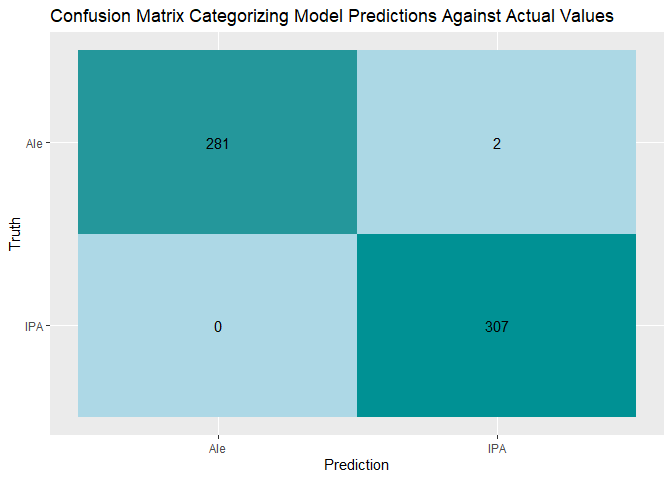
\includegraphics{ProjectMarkdown_files/figure-latex/unnamed-chunk-14-1.pdf}

\begin{Shaded}
\begin{Highlighting}[]
\FunctionTok{cat}\NormalTok{(}\StringTok{\textquotesingle{}Accuracy:\textquotesingle{}}\NormalTok{,CM}\SpecialCharTok{$}\NormalTok{overall[}\DecValTok{1}\NormalTok{]}\SpecialCharTok{*}\DecValTok{100}\NormalTok{,}\StringTok{"\%"}\NormalTok{,}
    \StringTok{"}\SpecialCharTok{\textbackslash{}n}\StringTok{Sensitivity:"}\NormalTok{,CM}\SpecialCharTok{$}\NormalTok{byClass[}\DecValTok{1}\NormalTok{]}\SpecialCharTok{*}\DecValTok{100}\NormalTok{, }\StringTok{"\%"}\NormalTok{,}
    \StringTok{"}\SpecialCharTok{\textbackslash{}n}\StringTok{Specificity:"}\NormalTok{,CM}\SpecialCharTok{$}\NormalTok{byClass[}\DecValTok{2}\NormalTok{]}\SpecialCharTok{*}\DecValTok{100}\NormalTok{, }\StringTok{"\%"}\NormalTok{)}
\end{Highlighting}
\end{Shaded}

\begin{verbatim}
Accuracy: 84.64 % 
Sensitivity: 90.16393 % 
Specificity: 76.83398 %
\end{verbatim}

\begin{Shaded}
\begin{Highlighting}[]
\DocumentationTok{\#\#\#\#\#\#\#\#\#\#\#\#\#\#\#\#\#\#\#\#\#\#\#\#\#\#\#\#\#\#\#\#\#\#\# KNN finding best K \#\#\#\#\#\#\#\#\#\#\#\#\#\#\#\#\#\#\#\#\#\#\#\#\#}

\NormalTok{iterations }\OtherTok{=} \DecValTok{50}
\NormalTok{num\_of\_k }\OtherTok{=} \DecValTok{50}
\NormalTok{split\_percent }\OtherTok{=}\NormalTok{ .}\DecValTok{3}

\NormalTok{model\_accuracy }\OtherTok{=} \FunctionTok{matrix}\NormalTok{(}\AttributeTok{nrow =}\NormalTok{ iterations, }\AttributeTok{ncol =}\NormalTok{ num\_of\_k)}
\NormalTok{model\_specificity }\OtherTok{=} \FunctionTok{matrix}\NormalTok{(}\AttributeTok{nrow =}\NormalTok{ iterations, }\AttributeTok{ncol =}\NormalTok{ num\_of\_k)}
\NormalTok{model\_sensitivity }\OtherTok{=} \FunctionTok{matrix}\NormalTok{(}\AttributeTok{nrow =}\NormalTok{ iterations, }\AttributeTok{ncol =}\NormalTok{ num\_of\_k)}

\ControlFlowTok{for}\NormalTok{ (j }\ControlFlowTok{in} \DecValTok{1}\SpecialCharTok{:}\NormalTok{iterations)}
\NormalTok{\{}
  \FunctionTok{set.seed}\NormalTok{(}\DecValTok{765}\NormalTok{)}
\NormalTok{  intrain2 }\OtherTok{\textless{}{-}} \FunctionTok{sample}\NormalTok{(}\FunctionTok{nrow}\NormalTok{(combine\_knn), }\FunctionTok{round}\NormalTok{(}\FunctionTok{nrow}\NormalTok{(combine\_knn)}\SpecialCharTok{*}\NormalTok{split\_percent))}
\NormalTok{  train2 }\OtherTok{\textless{}{-}}\NormalTok{ combine\_knn[intrain2,]}
\NormalTok{  test2 }\OtherTok{\textless{}{-}}\NormalTok{ combine\_knn[}\SpecialCharTok{{-}}\NormalTok{intrain2,]}
  \ControlFlowTok{for}\NormalTok{(i }\ControlFlowTok{in} \DecValTok{1}\SpecialCharTok{:}\NormalTok{num\_of\_k)}
\NormalTok{  \{}
\NormalTok{    classify }\OtherTok{=} \FunctionTok{knn}\NormalTok{(train2[,}\FunctionTok{c}\NormalTok{(}\DecValTok{3}\NormalTok{,}\DecValTok{4}\NormalTok{)],}
\NormalTok{                   test2[,}\FunctionTok{c}\NormalTok{(}\DecValTok{3}\NormalTok{,}\DecValTok{4}\NormalTok{)],}
\NormalTok{                   train2}\SpecialCharTok{$}\NormalTok{Style,}
                   \AttributeTok{k =}\NormalTok{ i, }\AttributeTok{prob =} \ConstantTok{TRUE}\NormalTok{)}
\NormalTok{    u }\OtherTok{=} \FunctionTok{union}\NormalTok{(classify, test2}\SpecialCharTok{$}\NormalTok{Style)}
\NormalTok{    t }\OtherTok{=} \FunctionTok{table}\NormalTok{(}\FunctionTok{factor}\NormalTok{(classify, u), }\FunctionTok{factor}\NormalTok{(test2}\SpecialCharTok{$}\NormalTok{Style, u))}
\NormalTok{    CM }\OtherTok{=} \FunctionTok{confusionMatrix}\NormalTok{(t)}
\NormalTok{    model\_accuracy[j,i] }\OtherTok{=}\NormalTok{ CM}\SpecialCharTok{$}\NormalTok{overall[}\DecValTok{1}\NormalTok{]}
\NormalTok{    model\_specificity[j,i] }\OtherTok{=}\NormalTok{ CM}\SpecialCharTok{$}\NormalTok{byClass[}\DecValTok{1}\NormalTok{]}
\NormalTok{    model\_sensitivity[j,i] }\OtherTok{=}\NormalTok{ CM}\SpecialCharTok{$}\NormalTok{byClass[}\DecValTok{2}\NormalTok{]}
\NormalTok{  \}}
  
  
\NormalTok{\}}

\NormalTok{mean\_accuracy }\OtherTok{=} \FunctionTok{colMeans}\NormalTok{(model\_accuracy)}
\CommentTok{\# to determine which level of k provided the best accuracy so that we can tune the model if needed}
\CommentTok{\# which.max(mean\_accuracy)}
\NormalTok{mean\_specificity }\OtherTok{=} \FunctionTok{colMeans}\NormalTok{(model\_specificity)}
\NormalTok{mean\_sensitivity }\OtherTok{=} \FunctionTok{colMeans}\NormalTok{(model\_sensitivity)}

\FunctionTok{plot}\NormalTok{(}\FunctionTok{seq}\NormalTok{(}\DecValTok{1}\NormalTok{,num\_of\_k,}\DecValTok{1}\NormalTok{),}
\NormalTok{     mean\_accuracy, }\AttributeTok{type =} \StringTok{"l"}\NormalTok{,}
     \AttributeTok{xlab =} \StringTok{"Kth value 1:50"}\NormalTok{,}
     \AttributeTok{ylab =} \StringTok{"Mean value of measured Accuracy"}\NormalTok{)}
\end{Highlighting}
\end{Shaded}

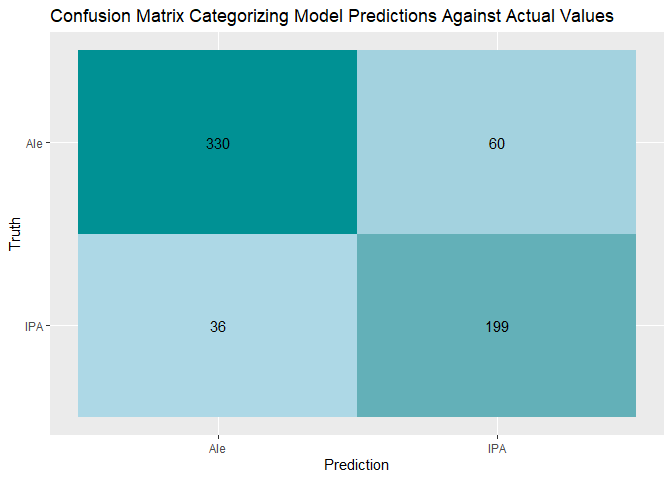
\includegraphics{ProjectMarkdown_files/figure-latex/unnamed-chunk-15-1.pdf}

\begin{Shaded}
\begin{Highlighting}[]
\FunctionTok{plot}\NormalTok{(}\FunctionTok{seq}\NormalTok{(}\DecValTok{1}\NormalTok{, num\_of\_k, }\DecValTok{1}\NormalTok{),}
\NormalTok{     mean\_specificity,}
     \AttributeTok{type =} \StringTok{\textquotesingle{}l\textquotesingle{}}\NormalTok{,}
     \AttributeTok{xlab =} \StringTok{"Kth value 1:50"}\NormalTok{,}
     \AttributeTok{ylab =} \StringTok{"Mean value of measured Specificity"}\NormalTok{)}
\end{Highlighting}
\end{Shaded}

\includegraphics{ProjectMarkdown_files/figure-latex/unnamed-chunk-15-2.pdf}

\begin{Shaded}
\begin{Highlighting}[]
\FunctionTok{plot}\NormalTok{(}\FunctionTok{seq}\NormalTok{(}\DecValTok{1}\NormalTok{, num\_of\_k, }\DecValTok{1}\NormalTok{),}
\NormalTok{     mean\_sensitivity, }\AttributeTok{type =} \StringTok{\textquotesingle{}l\textquotesingle{}}\NormalTok{,}
     \AttributeTok{xlab =} \StringTok{"Kth value 1:50"}\NormalTok{,}
     \AttributeTok{ylab =} \StringTok{"Mean value of measured Sensitivity"}\NormalTok{)}
\end{Highlighting}
\end{Shaded}

\includegraphics{ProjectMarkdown_files/figure-latex/unnamed-chunk-15-3.pdf}

\end{document}
